\documentclass[11pt]{article}

\usepackage[margin=0.82in]{geometry}
\usepackage[T1]{fontenc}
\usepackage[utf8]{inputenc}
\usepackage{lmodern}
\usepackage{microtype}
\usepackage{xcolor}
\usepackage{graphicx}
\usepackage{amsmath}
\usepackage{booktabs}
\usepackage{tabularx}
\usepackage{array}
\usepackage{enumitem}
\usepackage{float}
\usepackage[font=small,labelfont=bf,justification=raggedright,singlelinecheck=false]{caption}
\usepackage{xurl}
\usepackage{hyperref}
\usepackage{tikz}
\usetikzlibrary{arrows.meta, positioning, shapes.geometric, calc, fit, backgrounds}

\graphicspath{{figures/}}

\definecolor{Ink}{HTML}{17202A}
\definecolor{Muted}{HTML}{5E6B73}
\definecolor{Blue}{HTML}{2563EB}
\definecolor{Teal}{HTML}{0F766E}
\definecolor{Green}{HTML}{15803D}
\definecolor{Amber}{HTML}{B7791F}
\definecolor{Red}{HTML}{B91C1C}
\definecolor{Panel}{HTML}{F6F8FB}
\definecolor{Line}{HTML}{CBD5E1}
\definecolor{SoftBlue}{HTML}{DBEAFE}
\definecolor{SoftTeal}{HTML}{CCFBF1}
\definecolor{SoftGreen}{HTML}{DCFCE7}
\definecolor{SoftAmber}{HTML}{FEF3C7}
\definecolor{SoftRed}{HTML}{FEE2E2}
\definecolor{SoftGray}{HTML}{EEF2F7}

\hypersetup{
  colorlinks=true,
  linkcolor=Blue,
  urlcolor=Teal,
  citecolor=Blue,
  pdftitle={Human-Centered Laboratory Autonomy: AR-Guided Experiments, Scene-Level Learning, and Embodied Robot Integration},
  pdfauthor={Lachlan Chen, AgInTiFlow; AgInTi Lab, LazyingArt LLC}
}

\setlength{\parindent}{0pt}
\setlength{\parskip}{0.55em}
\setlist[itemize]{leftmargin=1.35em, topsep=0.2em, itemsep=0.1em}
\setlist[enumerate]{leftmargin=1.55em, topsep=0.2em, itemsep=0.1em}
\renewcommand{\arraystretch}{1.16}
\Urlmuskip=0mu plus 2mu
\emergencystretch=2em
\raggedbottom

\newcolumntype{Y}{>{\raggedright\arraybackslash}X}
\newcolumntype{L}[1]{>{\raggedright\arraybackslash}p{#1}}
\newcommand{\pill}[2]{%
  \tikz[baseline=(n.base)] \node[rounded corners=2pt, fill=#1, inner xsep=5pt, inner ysep=2pt] (n) {\footnotesize #2};%
}

\title{\vspace{-1.25cm}\textbf{Human-Centered Laboratory Autonomy}\\
\large AR-Guided Experiments, Scene-Level Learning, and Embodied Robot Integration}
\author{Lachlan Chen, AgInTiFlow\\AgInTi Lab, LazyingArt LLC\\\url{https://flow.lazying.art}}
\date{June 6, 2026}

\begin{document}
\maketitle
\vspace{-0.8em}

\begin{center}
\makebox[\linewidth][c]{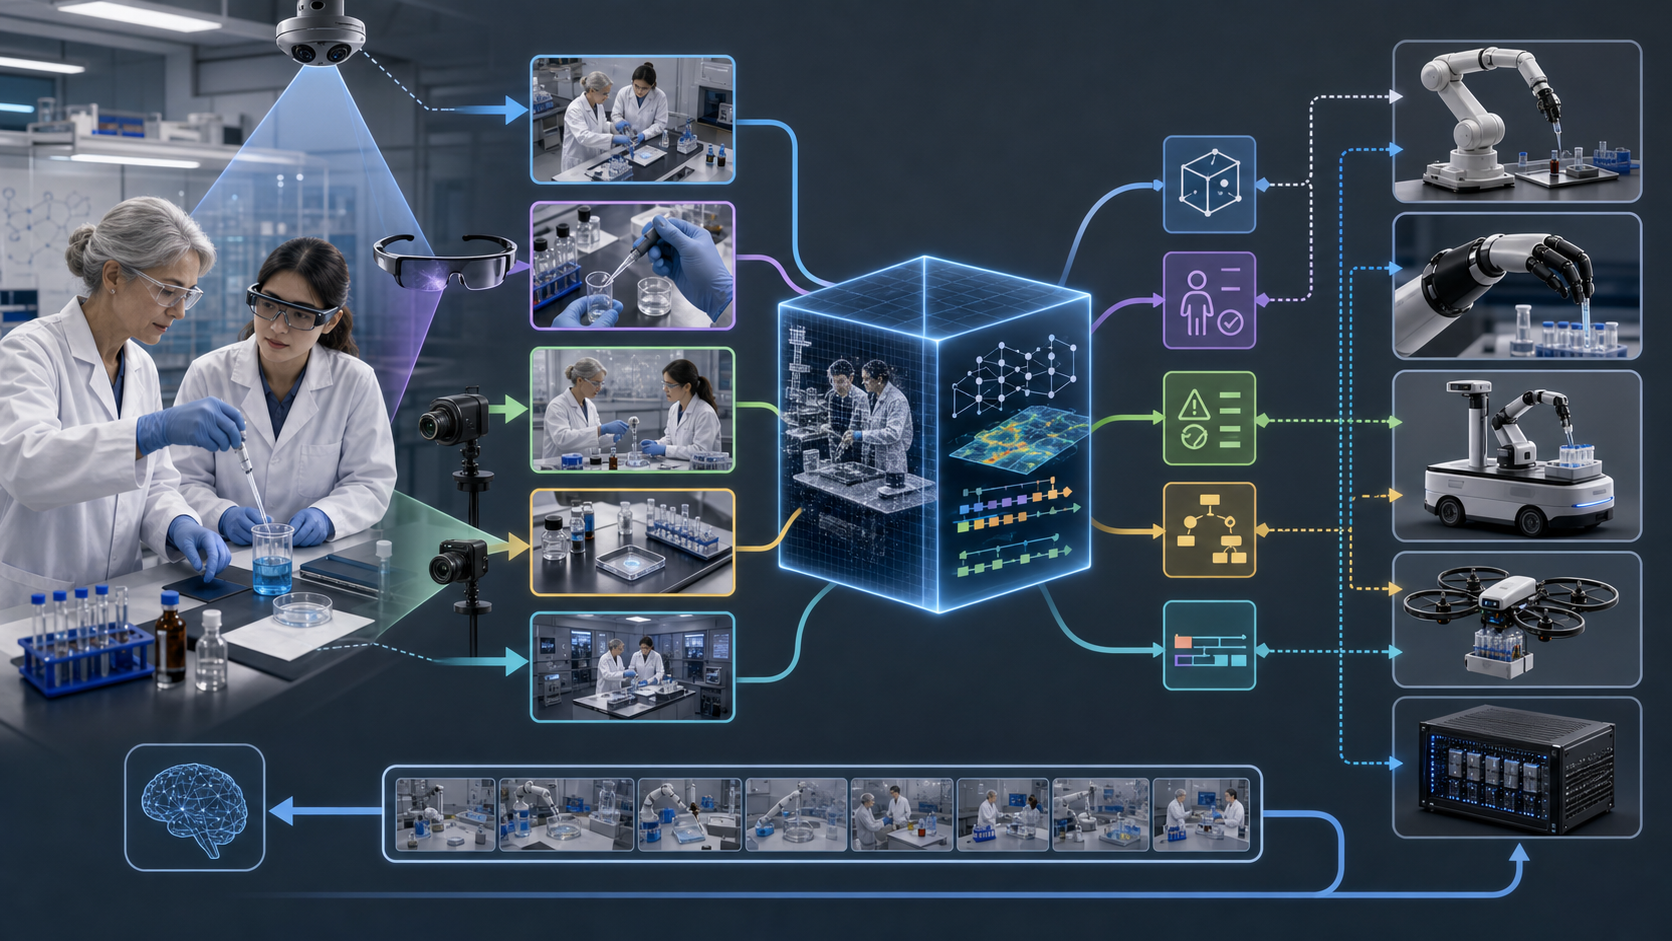
\includegraphics[width=1.08\linewidth,height=0.62\textheight,keepaspectratio]{scene_video_master_apprentice_training.png}}
\end{center}
\vfill
\newpage

\begin{abstract}
The strongest path to useful laboratory robotics is not to imitate the entire human body with a bionic hand, arm, eyes, legs, mobile base, and humanoid shell. The more feasible path is to treat the human laboratory worker as the current general-purpose embodiment, then build an autonomy stack around the worker: AR glasses for step guidance, cameras for scene understanding and quality control, robots for repetitive or hazardous actions, and shared AI models that learn from the full experimental scene. This report proposes a human-centered laboratory autonomy architecture in which the first product is an AR-and-camera experiment copilot, the second product is a robot-assist layer for constrained workcells, and the long-term product is a multi-embodiment operating system connecting humans, robot hands, robot arms, mobile bodies, drones, fixed instruments, and AI reasoning.
\end{abstract}

\tableofcontents
\newpage

\section{Executive Thesis}

If the goal is to reproduce the human hand, arm, eye, body, and foot, the first question should be: why not use the human being directly? The answer is not that robots are already better general laboratory workers. They are not. The answer is that humans and robots have different comparative advantages. Humans remain superior at flexible perception, improvisation, tacit judgement, and exception handling. Robots become valuable when the work is repetitive, hazardous, traceable, time-consuming, high-frequency, or physically constrained enough to be specified and validated.

The product direction is therefore not ``replace the scientist with a humanoid.'' It is ``turn the laboratory into an instrumented teaching and execution environment.'' In that environment, a senior person can teach a junior person, AR glasses can reduce working-memory load, cameras can create a structured record, and robots can gradually take over bounded actions after the system has learned the scene, protocol, risk, and decision points.

\textbf{Strategic claim.} The near-term wedge is an AR-guided experiment and camera-QA system for human operators. The medium-term wedge is a constrained robot-assist workcell that reuses the same scene graph and protocol engine. The long-term wedge is a master-apprentice learning platform where demonstrations are captured as synchronized scene videos, not merely as robot joint trajectories.

\begin{figure}[htbp]
\centering
\resizebox{\linewidth}{!}{%
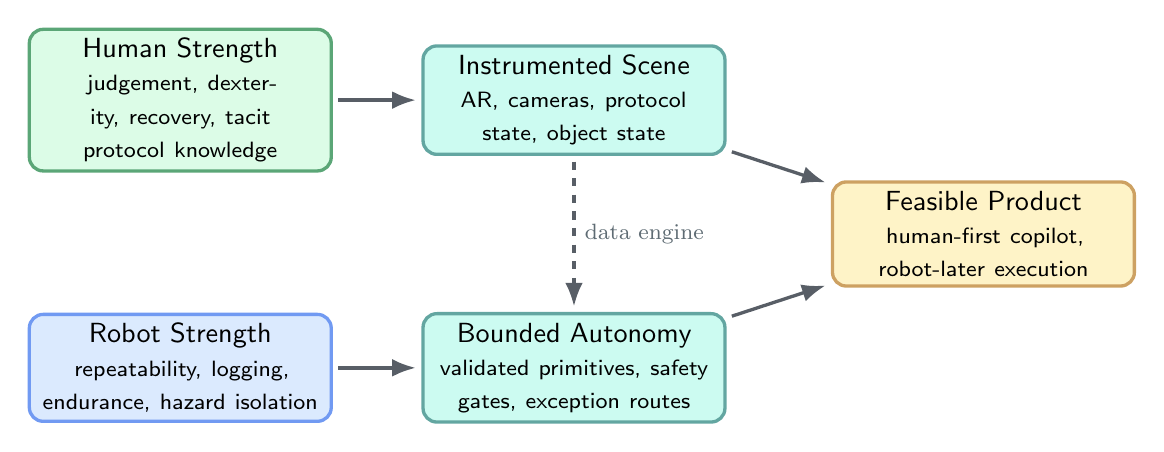
\begin{tikzpicture}[
  font=\sffamily,
  box/.style={rounded corners=5pt, draw=Line, very thick, align=center, minimum height=1.05cm, text width=3.6cm, fill=white},
  human/.style={box, fill=SoftGreen, draw=Green!70},
  robot/.style={box, fill=SoftBlue, draw=Blue!65},
  system/.style={box, fill=SoftTeal, draw=Teal!65},
  warn/.style={box, fill=SoftAmber, draw=Amber!70},
  arrow/.style={-{Latex[length=3mm]}, very thick, draw=Ink!72, shorten >=2pt, shorten <=2pt}
]
\node[human] (human) at (0,1.7) {Human Strength\\\footnotesize judgement, dexterity, recovery, tacit protocol knowledge};
\node[robot] (robot) at (0,-1.7) {Robot Strength\\\footnotesize repeatability, logging, endurance, hazard isolation};
\node[system] (scene) at (5.0,1.7) {Instrumented Scene\\\footnotesize AR, cameras, protocol state, object state};
\node[system] (policy) at (5.0,-1.7) {Bounded Autonomy\\\footnotesize validated primitives, safety gates, exception routes};
\node[warn] (product) at (10.2,0) {Feasible Product\\\footnotesize human-first copilot, robot-later execution};

\draw[arrow] (human) -- (scene);
\draw[arrow] (robot) -- (policy);
\draw[arrow] (scene) -- (product);
\draw[arrow] (policy) -- (product);
\draw[arrow, dashed] (scene) -- node[right, font=\footnotesize\color{Muted}] {data engine} (policy);
\end{tikzpicture}}
\caption{The central design principle is not human replacement. It is comparative advantage: humans teach and recover; robots execute validated tasks; the instrumented scene connects both.}
\label{fig:comparative-advantage}
\end{figure}

\section{Why Not Build A Bionic Human First?}

A bionic laboratory worker bundles many hard problems: hand dexterity, arm force control, active vision, navigation, balance, safety, tool use, semantic reasoning, chemical compatibility, cleaning, calibration, and protocol comprehension. Each component can be demonstrated in isolation, but the integrated system fails commercially if it cannot finish real protocols reliably inside ordinary labs.

\begin{table}[htbp]
\centering
\small
\begin{tabularx}{\linewidth}{@{}L{2.65cm}Y Y@{}}
\toprule
\textbf{Capability} & \textbf{Human baseline} & \textbf{Robot should be used when} \\
\midrule
Dexterous manipulation & Handles unusual objects, soft judgement, awkward bench layouts, and one-off recovery. & The action is repetitive, fixtureable, measurable, and can be verified by camera, scale, liquid level, or instrument output. \\
Visual understanding & Infers intent, context, risk, missing items, and ambiguous protocol meaning from messy scenes. & The scene can be converted into structured states: object identity, pose, container state, PPE state, step progress, and anomaly flags. \\
Mobility & Walks through existing labs, opens doors, changes tools, and adapts to clutter. & The payoff justifies mobile platforms, or the task is inventory, transport, inspection, or cross-instrument logistics. \\
Accountability & Signs off on judgement, safety, and deviations. & The system can log every action, sensor value, exception, decision, and human override. \\
Training & Senior workers teach juniors by demonstration, correction, and explanation. & Demonstrations can be recorded as synchronized scene data and converted into reusable protocol, perception, and policy assets. \\
\bottomrule
\end{tabularx}
\caption{The human body is the current general-purpose laboratory embodiment. Robotics should enter through narrow advantages, not through an attempt to copy the full human stack on day one.}
\label{tab:human-robot-comparison}
\end{table}

The conclusion is practical: start with the laboratory activity, not the robot morphology. A robot hand is useful only after the product knows what task matters, what failure looks like, what sensors can verify success, and what physical simplifications make the task reliable.

\section{Why Robots Still Matter}

Robots are still worth building because the laboratory has real work that humans should not have to perform manually forever. Their value is strongest in five cases.

\textbf{Repeatability.} Robots can perform the same validated primitive in the same coordinate frame, with the same timing and logged parameters. This matters for sample preparation, liquid handling, incubation transfer, imaging setup, and repetitive instrument loading.

\textbf{Endurance.} Robots do not get bored during night shifts, weekend runs, or long screening campaigns. A workcell can operate when the bottleneck is not creativity but sustained execution.

\textbf{Traceability.} A robotic or camera-mediated action can automatically produce an audit trail: object identity, plate map, reagent lot, transfer volume, time, image, exception, and operator intervention. Self-driving-lab literature increasingly emphasizes metrics, data completeness, and system characterization rather than raw autonomy claims \cite{volk2024metrics}.

\textbf{Hazard separation.} Robots can isolate humans from toxic reagents, repetitive strain, aerosols, heat, cold, radiation, or contamination risk. Safety must still be designed explicitly; recent SDL safety work warns that robotics can introduce new hazards if not instrumented and bounded \cite{sdl2025safety}.

\textbf{Data production.} A robot is also a data generator. Every attempt, success, failure, and correction can become training and process-improvement data if captured in a standardized scene model.

\section{The Gap Between Robot Demo And Real Lab Application}

The application gap is not just model intelligence. It is the compound effect of workflow specificity, safety, contamination control, fixtures, calibration, operator trust, economics, and integration with existing instruments. Many robotics demos show one impressive action; laboratory products must complete repeated protocols with acceptable exception rates.

\begin{table}[htbp]
\centering
\small
\begin{tabularx}{\linewidth}{@{}L{3.1cm}Y Y@{}}
\toprule
\textbf{Gap} & \textbf{Why it blocks deployment} & \textbf{Practical response} \\
\midrule
Protocol ambiguity & SOPs omit tacit judgement, visual checks, and exception rules. & Convert SOPs into step graphs with visual preconditions, expected observations, and escalation paths. \\
Scene variability & Containers, labels, instruments, lighting, hands, and occlusions change. & Use calibrated fixed cameras plus wearable views; build a lab-specific scene graph before policy autonomy. \\
Manipulation reliability & Transparent liquids, flexible tubes, caps, labels, gloves, and clutter create failure modes. & Start with fixtureable workflows and add cameras for labware state, liquid level, and completion checks. \\
Safety and compliance & Labs require PPE, hazard assessment, chemical hygiene practices, and human accountability. & Treat AR and robot plans as safety-gated assistance, not unbounded autonomy. \\
Economic proof & A general robot may be expensive while saving only small fragments of time. & Sell completed workflow reliability, reduced rework, faster training, and better records before selling hardware novelty. \\
\bottomrule
\end{tabularx}
\caption{The feasibility plan must close deployment gaps, not only improve the robot model.}
\label{tab:application-gap}
\end{table}

\section{Product Idea 1: AR-Guided Experiments}

The fastest useful product is AR guidance for human laboratory work. The interface should make experiments feel like a precise game: the next object glows, the target region is highlighted, the correct motion is shown, the timer starts automatically, and the system verifies completion through cameras and sensors. The goal is not to make the operator stop thinking. The goal is to remove unnecessary recall, search, and bookkeeping so the operator can focus on judgement and safety.

AR has supporting evidence but also a warning. Mixed-reality systems have been explored for chemical engineering lab training and workforce development \cite{teixeira2023ar}. At the same time, chemistry AR learning studies show that overlays can increase cognitive load if they are not designed carefully \cite{peeters2023ar}. Therefore, the design must be sparse, contextual, and action-oriented.

\begin{figure}[htbp]
\centering
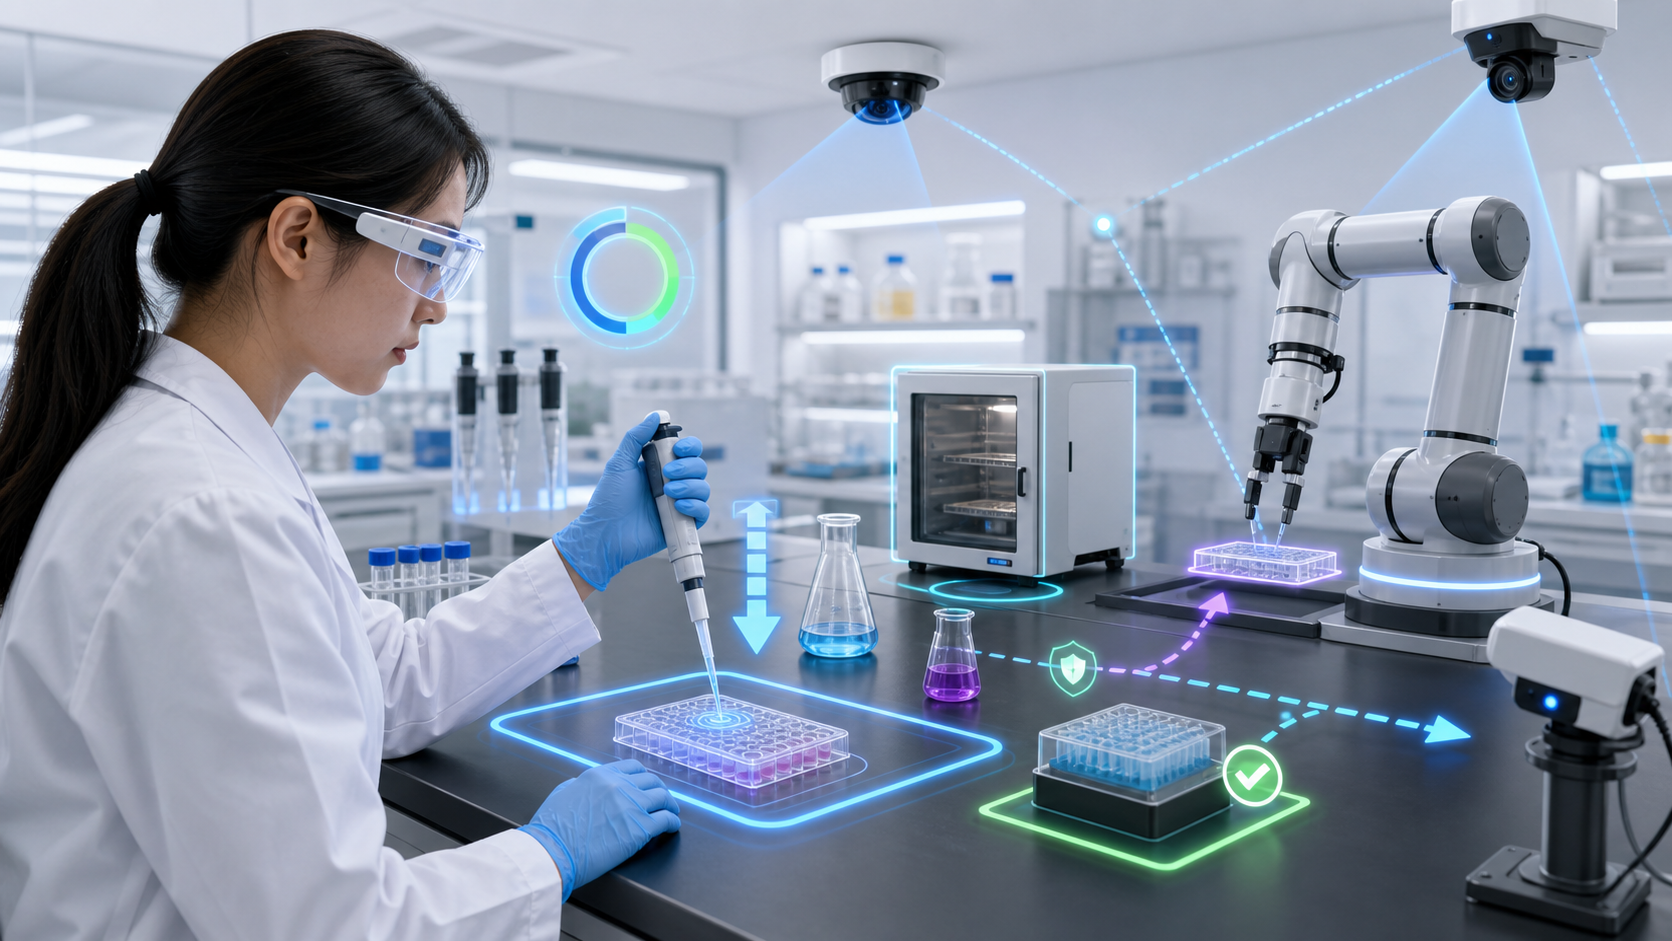
\includegraphics[width=\linewidth]{ar_guided_experiment_workflow.png}
\caption{AR-guided experiment concept. The operator sees spatial prompts, safe zones, progress markers, and object highlights while fixed cameras and robot-side cameras observe the same workspace for verification and later robot assistance.}
\label{fig:ar-guided-experiment}
\end{figure}

\textbf{Minimum viable workflow.} Choose one common workflow such as pipetting a plate, preparing a buffer, loading samples for imaging, or calibrating an instrument. Encode the SOP into a step graph. Each step has an expected object, location, timing, visual state, acceptable range, and failure recovery action.

\textbf{Operator experience.} The operator sees only the current step, the relevant object, and the next physical target. The interface should avoid dense text. Good AR guidance behaves like a cockpit: it presents the small amount of information needed at the exact time it is needed.

\textbf{Camera validation.} The camera layer checks that the right object is picked, the right plate region is used, the pipette is oriented plausibly, PPE is present, and the expected state change occurred. Recent work on vision-based recognition of pipetting operations shows the feasibility of using RGB/depth capture, object detection, pose features, and temporal models to identify standard and non-standard operations \cite{guo2026pipetting}.

\textbf{Immediate value.} This product can reduce training time, documentation burden, deviation ambiguity, and repeat errors before any robot is allowed to act. It also creates the data engine needed for future robot training.

\section{Product Idea 2: Camera-First Laboratory OS}

Current laboratories already contain many implicit visual checks: a person looks at color, turbidity, liquid level, container position, pipette state, plate occupancy, instrument state, cleanliness, label match, and PPE. A camera-first lab OS turns those visual checks into structured data. This does not require full robot autonomy at first.

\begin{figure}[htbp]
\centering
\resizebox{\linewidth}{!}{%
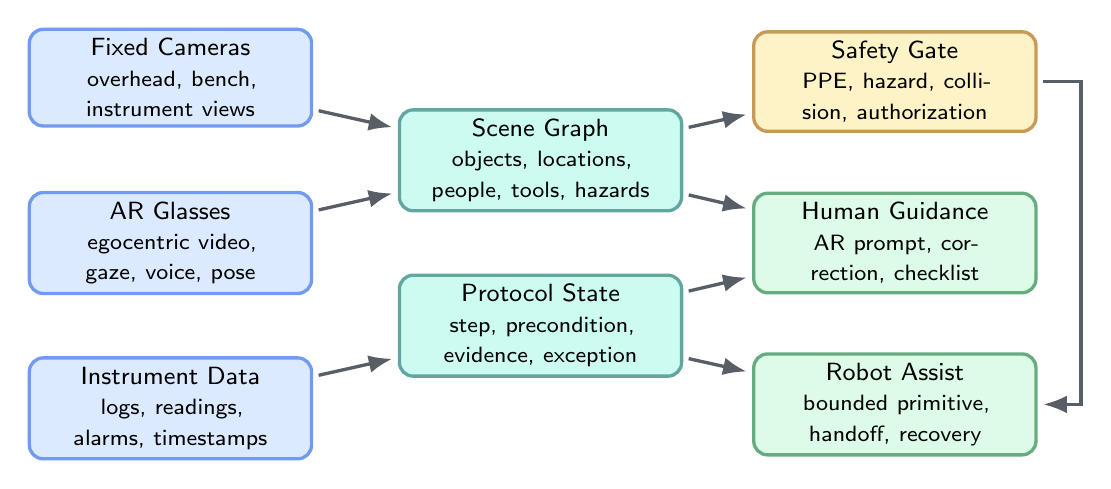
\begin{tikzpicture}[
  font=\sffamily\small,
  layer/.style={rounded corners=5pt, draw=Line, very thick, align=center, minimum height=1.05cm, text width=3.35cm, fill=white},
  sense/.style={layer, fill=SoftBlue, draw=Blue!65},
  state/.style={layer, fill=SoftTeal, draw=Teal!65},
  act/.style={layer, fill=SoftGreen, draw=Green!65},
  guard/.style={layer, fill=SoftAmber, draw=Amber!75},
  arrow/.style={-{Latex[length=3mm]}, very thick, draw=Ink!72, shorten >=2pt, shorten <=2pt}
]
\node[sense] (cams) at (0,2.1) {Fixed Cameras\\\footnotesize overhead, bench, instrument views};
\node[sense] (glasses) at (0,0) {AR Glasses\\\footnotesize egocentric video, gaze, voice, pose};
\node[sense] (instruments) at (0,-2.1) {Instrument Data\\\footnotesize logs, readings, alarms, timestamps};

\node[state] (scene) at (4.7,1.05) {Scene Graph\\\footnotesize objects, locations, people, tools, hazards};
\node[state] (protocol) at (4.7,-1.05) {Protocol State\\\footnotesize step, precondition, evidence, exception};

\node[guard] (safety) at (9.2,2.05) {Safety Gate\\\footnotesize PPE, hazard, collision, authorization};
\node[act] (ar) at (9.2,0) {Human Guidance\\\footnotesize AR prompt, correction, checklist};
\node[act] (robot) at (9.2,-2.05) {Robot Assist\\\footnotesize bounded primitive, handoff, recovery};

\draw[arrow] (cams) -- (scene);
\draw[arrow] (glasses) -- (scene);
\draw[arrow] (instruments) -- (protocol);
\draw[arrow] (scene) -- (safety);
\draw[arrow] (scene) -- (ar);
\draw[arrow] (protocol) -- (ar);
\draw[arrow] (protocol) -- (robot);
\draw[arrow] (safety.east) -- ++(0.55,0) |- (robot.east);
\end{tikzpicture}}
\caption{Camera-first laboratory OS. The first software product is not a robot brain; it is a shared scene and protocol state that can guide humans and safely constrain robot assistance.}
\label{fig:camera-os}
\end{figure}

This direction is supported by multiple recent examples. Computer vision has been used for real-time monitoring and control of chemical workups, including liquid level, turbidity, homogeneity, solids, residue, and color \cite{elkhawaldeh2024eye}. OT2Eye uses images and videos from an Opentrons OT-2 to detect labware type, position, and tip state \cite{ot2eye2026}. Chemist Eye uses distributed RGB, depth, and infrared cameras with a VLM to monitor PPE, fire hazards, and robot-relevant safety decisions in a self-driving laboratory \cite{chemistEye2026}.

The practical implication is simple: cameras are not an accessory. They are the bridge between human work, robot work, training data, and auditability.

\section{Product Idea 3: Scene-Video Training Instead Of Hand-Only Training}

Traditional robot learning often focuses on the hand, gripper, joint states, or end-effector trajectory. That is necessary but incomplete. A laboratory task is not just a hand path. It is a situated decision process: which sample, which tool, which step, which safety constraint, which exception, which visual evidence, which instruction, and which recovery action.

Recent robotics work points in the right direction. RT-2 framed robot control as a vision-language-action problem where visual and language pretraining can transfer into action \cite{rt2}. Open X-Embodiment assembled data from many robots and skills, showing that cross-robot training can transfer experience \cite{openx}. DROID emphasized diverse in-the-wild manipulation data across many scenes and tasks \cite{droid}. OpenVLA released an open VLA model trained on a large set of real-world robot demonstrations \cite{openvla}. More recent work such as $\pi_{0.5}$ and Qwen-VLA explicitly points toward heterogeneous data, high-level semantic prediction, robot embodiment descriptions, human egocentric demonstrations, and cross-task generalization \cite{pi05,qwenvla}.

The proposed training method is therefore scene-first:

\begin{enumerate}
  \item Record senior-to-junior teaching sessions with synchronized fixed cameras, AR-glasses egocentric video, voice, gaze if available, instrument logs, and final result data.
  \item Segment the session into protocol phases, object states, operator intents, safety checkpoints, action choices, mistakes, corrections, and completion evidence.
  \item Train a scene model to answer questions such as: What step is being performed? What object matters now? What risk is present? What evidence confirms completion? What should the next action be?
  \item Only then train robot-specific policies for bounded physical primitives that are grounded in the scene model.
\end{enumerate}

\begin{figure}[htbp]
\centering
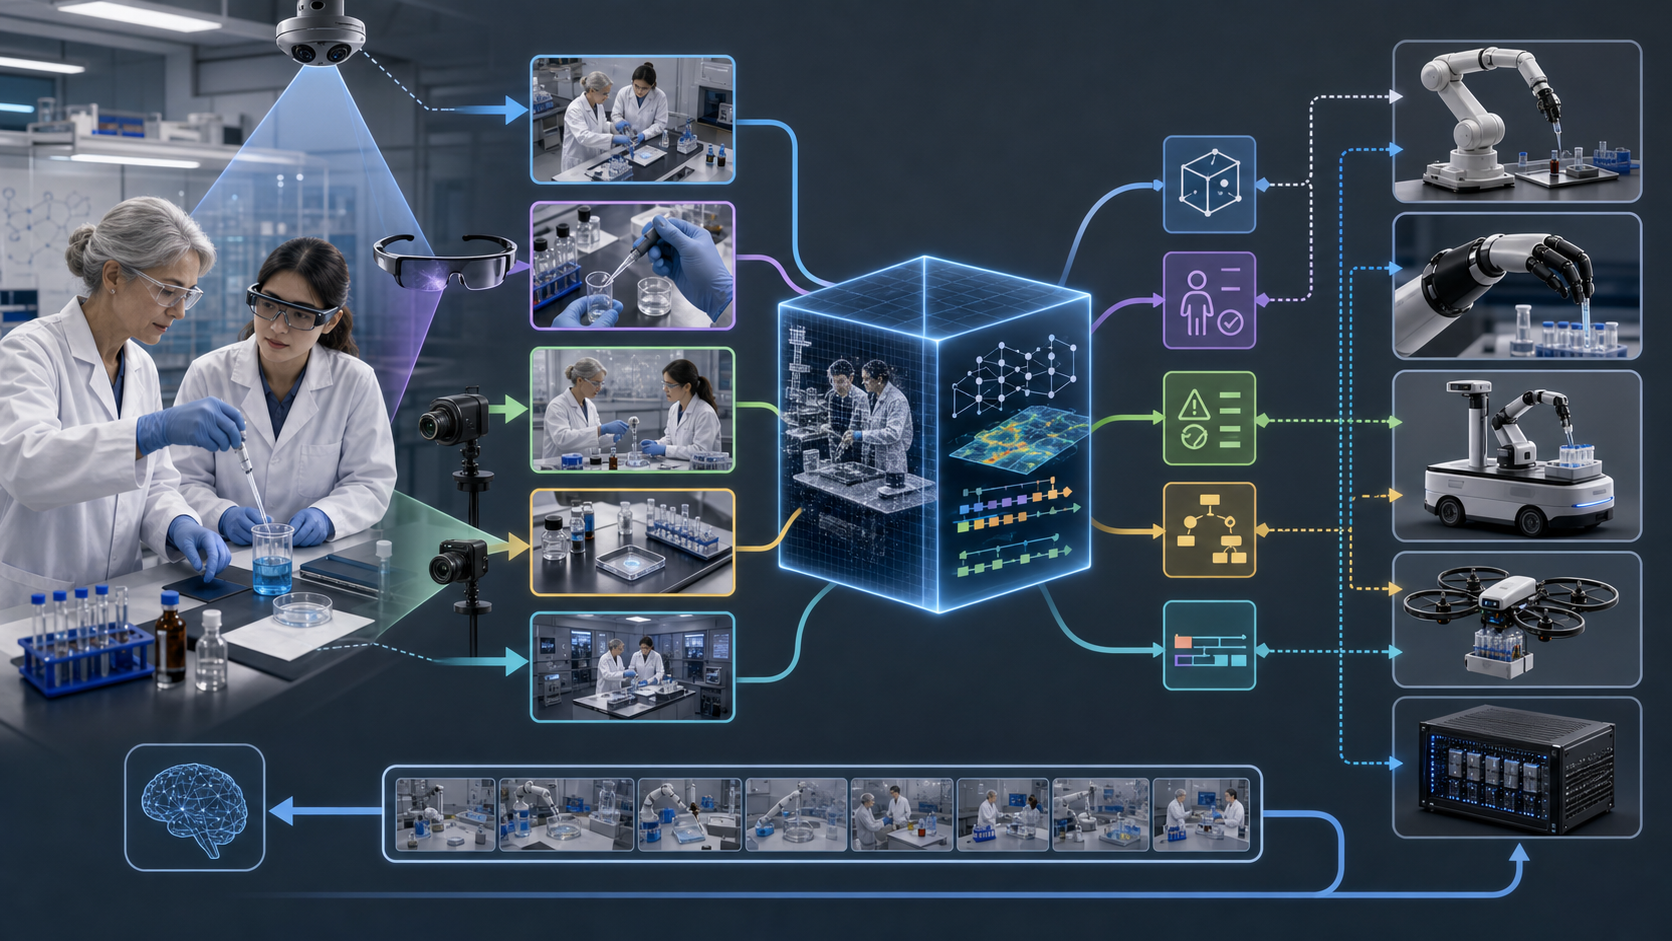
\includegraphics[width=\linewidth]{scene_video_master_apprentice_training.png}
\caption{Master-apprentice scene-video training concept. The core data object is not only a robot trajectory; it is synchronized human demonstration, scene context, instruction, correction, safety state, and action evidence that can later condition multiple robot embodiments.}
\label{fig:scene-video-training}
\end{figure}

The key advantage is transfer. If the system understands the scene and protocol state, then a robot hand, robot arm, mobile body, drone, or AR-guided human can all be treated as different executors of the same task graph. The action details differ, but the situational understanding is shared.

\section{Master-Apprentice Learning Loop}

The senior-junior teaching pattern is a natural data engine. Senior workers already explain why a step matters, what to check, what can go wrong, and how to recover. A good system captures that teaching signal instead of throwing it away.

\begin{figure}[htbp]
\centering
\resizebox{\linewidth}{!}{%
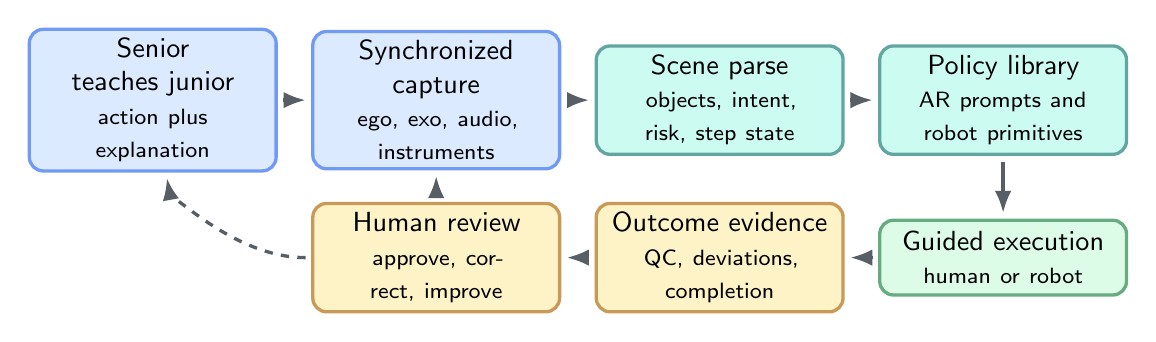
\begin{tikzpicture}[
  font=\sffamily,
  stage/.style={rounded corners=5pt, draw=Line, very thick, align=center, minimum height=0.95cm, text width=2.9cm, fill=white},
  data/.style={stage, fill=SoftBlue, draw=Blue!65},
  model/.style={stage, fill=SoftTeal, draw=Teal!65},
  exec/.style={stage, fill=SoftGreen, draw=Green!65},
  eval/.style={stage, fill=SoftAmber, draw=Amber!75},
  arrow/.style={-{Latex[length=2.8mm]}, very thick, draw=Ink!72, shorten >=2pt, shorten <=2pt}
]
\node[data] (teach) at (0,0) {Senior teaches junior\\\footnotesize action plus explanation};
\node[data] (capture) at (3.6,0) {Synchronized capture\\\footnotesize ego, exo, audio, instruments};
\node[model] (parse) at (7.2,0) {Scene parse\\\footnotesize objects, intent, risk, step state};
\node[model] (policy) at (10.8,0) {Policy library\\\footnotesize AR prompts and robot primitives};
\node[exec] (deploy) at (10.8,-2.0) {Guided execution\\\footnotesize human or robot};
\node[eval] (qa) at (7.2,-2.0) {Outcome evidence\\\footnotesize QC, deviations, completion};
\node[eval] (review) at (3.6,-2.0) {Human review\\\footnotesize approve, correct, improve};

\draw[arrow] (teach) -- (capture);
\draw[arrow] (capture) -- (parse);
\draw[arrow] (parse) -- (policy);
\draw[arrow] (policy) -- (deploy);
\draw[arrow] (deploy) -- (qa);
\draw[arrow] (qa) -- (review);
\draw[arrow] (review) -- (capture);
\draw[arrow, dashed] (review) .. controls (1.0,-2.0) and (0.2,-1.1) .. (teach);
\end{tikzpicture}}
\caption{Master-apprentice loop. Each teaching session becomes a reusable asset: demonstration video, explanation, protocol segmentation, safety labels, action evidence, and correction history.}
\label{fig:master-apprentice-loop}
\end{figure}

The loop should be designed as a product, not merely a data collection project. The senior should be able to correct a step label, approve a suggested rule, record an exception, and mark a demonstration as canonical. The junior should receive better AR prompts after every reviewed demonstration. The robot should only receive a primitive when the scene state and safety gate are known.

\section{Integrated Embodiment Architecture}

The final system should connect AI, humans, robot hands, robot arms, mobile bases, drones, fixed cameras, instruments, and AR glasses. The architecture should not assume that every embodiment is useful for every protocol. Instead, each embodiment should expose a capability contract.

\begin{table}[htbp]
\centering
\small
\begin{tabularx}{\linewidth}{@{}L{2.4cm}Y Y@{}}
\toprule
\textbf{Embodiment} & \textbf{Useful role} & \textbf{Do not use it for} \\
\midrule
Human operator & Flexible handling, judgement, exception recovery, teaching demonstrations, final sign-off. & High-frequency repetitive steps that can be verified and automated cheaply. \\
AR glasses & Step prompts, visual targeting, hands-free checklists, egocentric capture, voice notes, remote supervision. & Dense dashboards, long text, or overlays that block PPE, peripheral vision, or safety awareness. \\
Fixed cameras & Scene state, labware checks, PPE checks, liquid and object monitoring, audit evidence. & Private areas or unbounded recording without governance and retention rules. \\
Robot hand/arm & Fixtureable manipulation, transfers, plate handling, instrument loading, repetitive setup. & Unbounded chemical improvisation or ambiguous manipulation without human approval. \\
Mobile body/foot & Transport, inventory, instrument-to-instrument logistics, inspection routes. & First product in a small bench workflow where mobility adds cost but little value. \\
Drone & Shelf inspection, inventory scan, remote visual check in large facilities if allowed by safety policy. & Wet-bench manipulation, airflow-sensitive work, or crowded human areas. \\
AI model & Scene parsing, protocol state, safety triage, next-step suggestion, data mining, policy selection. & Unreviewed autonomous action in hazardous or regulated steps. \\
\bottomrule
\end{tabularx}
\caption{Embodiments should be connected through capability contracts. The system assigns work to the executor with the best cost, safety, and reliability profile for the current step.}
\label{tab:embodiments}
\end{table}

The shared interface is the protocol-scene graph. Each node represents a state or action: object detected, reagent verified, PPE present, plate positioned, liquid transferred, incubation complete, readout captured, anomaly flagged. Humans and robots read and write to the same graph, but with different permissions.

\section{MVP Demo Scenario}

The first public demo should be a real laboratory workflow that is visually understandable, safe to run repeatedly, and rich enough to show why AR glasses, AI, robots, drones, cameras, and the lab environment belong in one system. A strong MVP is an \textbf{AR-guided sample intake and 96-well plate preparation demo} using non-hazardous colored liquids or a low-risk training assay. The demo should not try to prove full autonomy. It should prove coordinated autonomy: every executor sees the same protocol state, every action creates evidence, and the system can stop or redirect work when the scene is wrong.

\textbf{Demo story.} A junior operator enters the lab wearing AR glasses. The AI identifies the operator, confirms PPE, loads the protocol, and highlights the correct rack, plate, pipette, reagent bottle, and target wells. Fixed cameras watch the bench. A drone performs a short inventory scan of sealed shelves or a marked storage aisle to locate the required closed reagent box; it does not fly over open liquids, people, or active bench work. A mobile robot or human receives the located item. The operator follows AR prompts to prepare the plate. The camera model verifies each checkpoint. A robot arm then moves the closed plate to a reader, incubator, or imaging station. The system produces a complete run record: protocol step, object evidence, operator confirmation, robot action, inventory source, deviations, and final result image.

\begin{figure}[htbp]
\centering
\resizebox{\linewidth}{!}{%
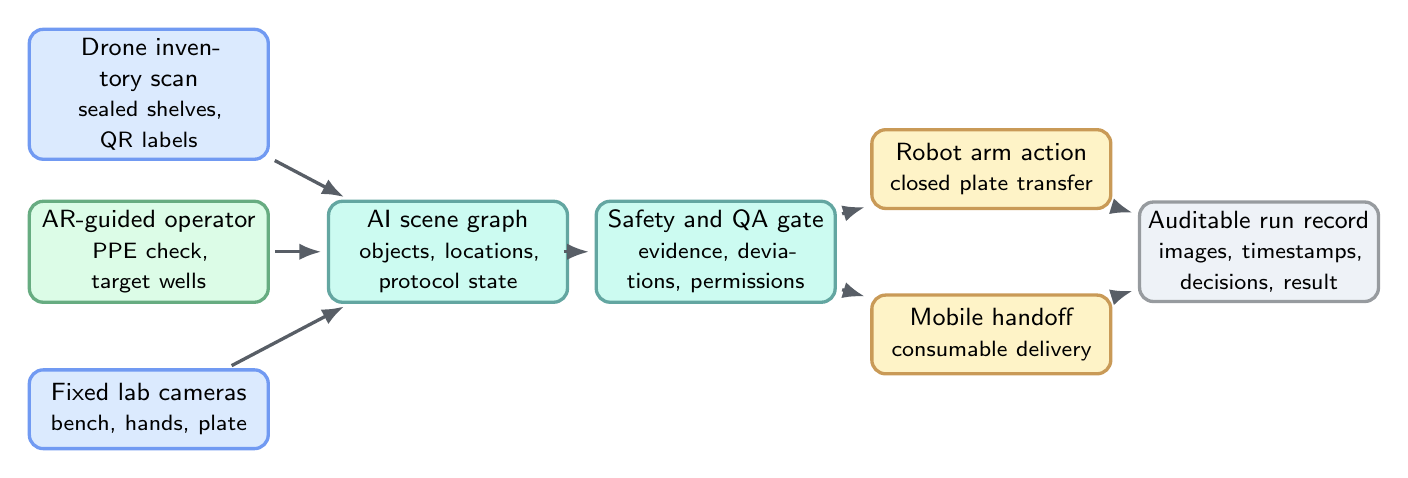
\begin{tikzpicture}[
  font=\sffamily\small,
  nodebox/.style={rounded corners=5pt, draw=Line, very thick, align=center, minimum height=1.0cm, text width=2.8cm, fill=white},
  human/.style={nodebox, fill=SoftGreen, draw=Green!65},
  sense/.style={nodebox, fill=SoftBlue, draw=Blue!65},
  ai/.style={nodebox, fill=SoftTeal, draw=Teal!65},
  robot/.style={nodebox, fill=SoftAmber, draw=Amber!75},
  outputbox/.style={nodebox, fill=SoftGray, draw=Ink!45},
  arrow/.style={-{Latex[length=2.8mm]}, very thick, draw=Ink!72, shorten >=2pt, shorten <=2pt}
]
\node[sense] (drone) at (0,2.0) {Drone inventory scan\\\footnotesize sealed shelves, QR labels};
\node[human] (ar) at (0,0) {AR-guided operator\\\footnotesize PPE check, target wells};
\node[sense] (cams) at (0,-2.0) {Fixed lab cameras\\\footnotesize bench, hands, plate};

\node[ai] (scene) at (3.8,0) {AI scene graph\\\footnotesize objects, locations, protocol state};
\node[ai] (gate) at (7.2,0) {Safety and QA gate\\\footnotesize evidence, deviations, permissions};

\node[robot] (arm) at (10.7,1.05) {Robot arm action\\\footnotesize closed plate transfer};
\node[robot] (mobile) at (10.7,-1.05) {Mobile handoff\\\footnotesize consumable delivery};
\node[outputbox] (record) at (14.1,0) {Auditable run record\\\footnotesize images, timestamps, decisions, result};

\draw[arrow] (drone) -- (scene);
\draw[arrow] (ar) -- (scene);
\draw[arrow] (cams) -- (scene);
\draw[arrow] (scene) -- (gate);
\draw[arrow] (gate) -- (arm);
\draw[arrow] (gate) -- (mobile);
\draw[arrow] (arm) -- (record);
\draw[arrow] (mobile) -- (record);
\end{tikzpicture}}
\caption{MVP demo flow. The first demo should show coordinated autonomy across AR guidance, camera QA, AI scene state, drone inventory, robot transfer, and a complete experimental record.}
\label{fig:mvp-demo}
\end{figure}

\textbf{Why this scenario is strong.} It is easy for an audience to understand because the plate, colored wells, AR highlights, drone shelf scan, robot transfer, and final plate image are visible. It is safe because hazardous chemistry is not needed. It is technically honest because the human still performs the dexterous wet step, while the robot handles bounded transfer and the drone handles inventory observation. It is commercially relevant because training, sample prep, inventory, instrument loading, and documentation are common laboratory pain points.

\begin{table}[htbp]
\centering
\small
\begin{tabularx}{\linewidth}{@{}L{2.55cm}Y Y@{}}
\toprule
\textbf{MVP component} & \textbf{First-demo role} & \textbf{Success criterion} \\
\midrule
AR glasses & Show the operator what to pick, where to pipette, when to wait, and when to confirm. & Operator completes the plate with fewer visible hesitations and without reading a paper SOP. \\
AI scene model & Maintain a shared state of operator, PPE, rack, reagent, plate, well targets, inventory, and instrument status. & The system can explain the current step and identify the next valid action. \\
Fixed cameras & Verify object presence, hand/tool location, plate position, and selected error cases. & At least three important checkpoints are verified from video evidence. \\
Drone & Scan sealed shelves or storage aisle for the required closed reagent/consumable box. & The system locates the item and updates the scene graph without entering the wet-bench zone. \\
Robot arm & Move only closed, fixtureable items: plate carrier, sealed plate, or rack. & The robot completes a bounded transfer only after the safety gate approves it. \\
Run record & Combine AR confirmations, camera evidence, drone inventory result, robot action, and final image. & A PDF or dashboard entry is produced automatically at the end of the run. \\
\bottomrule
\end{tabularx}
\caption{MVP scope. Each component has a visible role and a clear pass/fail criterion, preventing the demo from becoming a vague robotics showcase.}
\label{tab:mvp-scope}
\end{table}

\textbf{Demo failure moment.} The demo should include one intentional recoverable mistake: the wrong tube is placed in the rack, the plate is rotated, or the operator reaches toward the wrong well column. The AR overlay should pause the step, the camera model should provide evidence, and the robot should refuse downstream transfer until the correction is made. This single moment communicates the product better than a perfectly scripted run.

\textbf{Build target.} The MVP can be built without a general humanoid. The minimum hardware is one AR device or tablet fallback, two fixed cameras, one small robot arm with a plate fixture, one indoor drone restricted to a marked inventory path or safety cage, and one workstation running the protocol-state service. The software target is one protocol, one scene graph, one reviewable run record, and five reliable checks: PPE present, correct rack, correct plate orientation, correct target region, and closed-plate transfer allowed.

\section{Feasibility Roadmap}

The feasible path is staged. Do not begin by building a humanoid. Begin by making human work observable, structured, and easier. Then automate only the steps where the product has proof.

\begin{table}[htbp]
\centering
\scriptsize
\begin{tabularx}{\linewidth}{@{}L{1.8cm}L{2.8cm}Y Y Y@{}}
\toprule
\textbf{Phase} & \textbf{Build} & \textbf{Proof metric} & \textbf{Main risk} & \textbf{Exit condition} \\
\midrule
0. Bench selection & Pick one protocol family, one lab layout, one operator group. & Protocol repeated at least 30 times with visible state changes and measurable outcomes. & Choosing a workflow too broad or too low value. & A signed workflow spec with steps, objects, evidence, and failure modes. \\
1. AR copilot & Step graph, AR prompts, voice notes, basic camera capture. & Training time, step error rate, missing documentation, operator acceptance. & AR overload or PPE conflict. & Operators prefer guided mode for routine runs. \\
2. Camera QA & Fixed camera calibration, object detection, action segmentation, anomaly flags. & False positive/negative rates, detected deviations, review time saved. & Occlusion and lighting variability. & Camera evidence is trusted for selected checkpoints. \\
3. Robot assist & Add one bounded primitive such as plate transfer, tip-rack check, or instrument loading. & Completion rate, exception rate, human intervention rate, cycle time. & Hardware integration and safety validation. & Robot primitive runs under safety gate with repeatable benefit. \\
4. Scene policy & Train scene model from master-apprentice sessions and reviewed runs. & Step recognition, next-action accuracy, exception triage, transfer to new users. & Data quality and causal ambiguity. & Model improves AR prompts and chooses robot-assist opportunities. \\
5. Multi-embodiment OS & Capability contracts for arms, hands, mobile base, drones, instruments, and humans. & Cross-executor task handoff, audit completeness, ROI by workflow. & Architecture breadth before workflow depth. & Two or more executors complete a protocol segment through the same scene graph. \\
\bottomrule
\end{tabularx}
\caption{Feasibility roadmap from human-first guidance to bounded robot autonomy. Each phase produces a deployable asset even if later phases take longer.}
\label{tab:roadmap}
\end{table}

\section{Prototype Design}

The first prototype should use ordinary equipment wherever possible:

\begin{itemize}
  \item one fixed overhead RGB or RGB-D camera;
  \item one side camera focused on hands, pipette, tube rack, plate, and work zone;
  \item optional AR glasses or a tablet fallback for early testing;
  \item a protocol engine that represents steps, preconditions, expected visual evidence, timers, and deviations;
  \item a local review tool for labeling step boundaries, object states, mistakes, and corrections;
  \item a simple dashboard for completed runs, deviations, and training examples.
\end{itemize}

The first model does not need to solve general robotics. It needs to solve narrow questions reliably:

\begin{itemize}
  \item Is the correct plate or tube rack present?
  \item Is the operator at the correct step?
  \item Did the expected object move to the expected region?
  \item Is PPE visible when the step requires it?
  \item Is there a visible anomaly such as missing tip, wrong container, spill, empty rack, or unexpected pause?
  \item Is this step ready for human confirmation or robot execution?
\end{itemize}

This prototype creates a valuable product even before a robot is added. It improves training, documentation, and process consistency. It also creates the dataset that later makes robot assistance less speculative.

\section{Model Strategy}

The model stack should be layered rather than monolithic.

\textbf{Layer 1: perception.} Object detection, hand/tool pose, labware state, PPE state, liquid level, color, turbidity, and instrument display state. Some of these can be conventional models; not every sensor needs a large model.

\textbf{Layer 2: temporal state.} Step recognition, action segmentation, deviation detection, and completion evidence. Vision-based pipetting work shows why temporal models are important: a single frame is often insufficient, while sequence context can distinguish standard and non-standard behavior \cite{guo2026pipetting}.

\textbf{Layer 3: scene-language reasoning.} A VLM/VLA-style model interprets instructions, visual context, risk, and next-step logic. It should explain uncertainty and ask for confirmation at safety boundaries.

\textbf{Layer 4: action interface.} AR prompts, human checklists, robot primitives, instrument API calls, and notification actions. This layer must be permissioned; the model proposes, but safety gates decide what is allowed.

\textbf{Layer 5: continuous improvement.} Every reviewed run updates prompt design, protocol rules, perception labels, and future robot candidate steps. The 2026 VLA data-engine survey argues that progress depends heavily on data infrastructure, benchmarks, and scalable data generation, not only model architecture \cite{vlasurvey2026}.

\section{Safety, Privacy, And Governance}

AR glasses and cameras create value by observing the lab, but observation also creates governance obligations. The product should include clear retention settings, privacy zones, user consent, role-based access, and redaction where needed. It should avoid recording private areas and should allow labs to keep sensitive data local.

Safety must be treated as a first-class product feature. OSHA laboratory guidance emphasizes chemical hygiene, safety culture, hazard recognition, and standards for non-production laboratories \cite{oshaLabs}. CDC/NIOSH guidance highlights fit, coverage, peripheral vision, and appropriate eye protection for the hazard \cite{nioshEye}. AR glasses must therefore be compatible with required PPE and should never block peripheral awareness or encourage unsafe shortcuts.

Robot actions should be gated by:

\begin{itemize}
  \item verified scene preconditions;
  \item allowed chemical and biological risk class;
  \item human presence and separation state;
  \item emergency stop and physical limits;
  \item instrument state and interlocks;
  \item auditable human approval for non-routine actions.
\end{itemize}

\section{Business Direction}

The commercial positioning should avoid the phrase ``general humanoid scientist'' as the first product. It creates expectations the system cannot meet. A stronger first offer is:

\begin{center}
\fbox{\parbox{0.91\linewidth}{\centering
\textbf{An AR-and-camera laboratory copilot that trains operators, verifies protocol execution, creates structured experimental records, and identifies the exact steps ready for robot assistance.}}}
\end{center}

This wedge can be sold to research labs, core facilities, CROs, process-development teams, and teaching laboratories. The value proposition is faster onboarding, fewer repeated mistakes, better records, easier supervision, and a future robot path grounded in real workflow data.

The second offer is a robot-assist module for one proven workflow. The company should add hardware only after the camera and AR system has measured enough repetitions to prove where automation pays.

\section{Next Actionable Steps}

\begin{enumerate}
  \item Select one workflow with high repetition and visible state changes: pipetting plate setup, buffer preparation, sample loading, or imaging preparation.
  \item Film 20--30 master-apprentice demonstrations with at least two fixed cameras and one egocentric view.
  \item Convert the SOP into a step graph with preconditions, expected evidence, deviations, and escalation rules.
  \item Build a minimal AR or tablet guidance interface with object highlights, timer checkpoints, and completion confirmations.
  \item Train a narrow camera-QA model for 3--5 visual checks that matter commercially.
  \item Measure error rate, training time, review time, and documentation completeness before and after guidance.
  \item Use the run log to rank robot-assist candidates by frequency, risk, fixtureability, sensor-verifiability, and ROI.
  \item Add one robot primitive only after the product can prove scene readiness and verify completion.
\end{enumerate}

\section{Conclusion}

The feasible route to laboratory autonomy is human-centered, scene-centered, and evidence-centered. The system should use the human body where general intelligence and dexterity are still unmatched. It should use AR glasses to make human work easier and more consistent. It should use cameras to transform implicit visual judgement into structured records. It should use robots where repetition, safety, endurance, and traceability justify the complexity. It should train models from the whole scene and teaching process, not only from robot hand trajectories.

This strategy creates a practical ladder: human guidance first, camera QA second, bounded robot assist third, scene-level policy learning fourth, and multi-embodiment autonomy only after the earlier layers have earned trust.

\begin{thebibliography}{99}
\raggedright
\small

\bibitem{abolhasani2023rise}
Milad Abolhasani and Eugenia Kumacheva.
The rise of self-driving labs in chemical and materials sciences.
\emph{Nature Synthesis}, 2023.
\url{https://www.nature.com/articles/s44160-022-00231-0}

\bibitem{volk2024metrics}
Amanda A. Volk and Milad Abolhasani.
Performance metrics to unleash the power of self-driving labs in chemistry and materials science.
\emph{Nature Communications}, 2024.
\url{https://www.nature.com/articles/s41467-024-45569-5}

\bibitem{sdl2025safety}
Steering towards safe self-driving laboratories.
\emph{Nature Reviews Chemistry}, 2025.
\url{https://www.nature.com/articles/s41570-025-00747-x}

\bibitem{guo2026pipetting}
Chuntao Guo, Jing Lin, Shunxing Bao, Xin Liu, Yaru Wang, and Yunlin Chen.
A Vision-Based Deep Learning Framework for Monitoring and Recognition of Chemical Laboratory Operations.
\emph{Sensors}, 2026.
\url{https://www.mdpi.com/1424-8220/26/4/1106}

\bibitem{ot2eye2026}
OT2Eye: Detection of labware conditions to monitor and extend affordable liquid-handling robots.
\emph{SLAS Technology}, 2026.
\url{https://www.sciencedirect.com/science/article/pii/S2472630326000233}

\bibitem{chemistEye2026}
Francisco Munguia-Galeano, Zhengxue Zhou, Satheeshkumar Veeramani, Hatem Fakhruldeen, Louis Longley, Rob Clowes, and Andrew I. Cooper.
Chemist Eye: a visual language model-powered system for safety monitoring and robot decision-making in self-driving laboratories.
\emph{Digital Discovery}, 2026.
\url{https://pubs.rsc.org/en/content/articlelanding/2026/dd/d6dd00062b}

\bibitem{elkhawaldeh2024eye}
Rama El-khawaldeh et al.
Keeping an eye on the experiment: computer vision for real-time monitoring and control.
\emph{Chemical Science}, 2024.
\url{https://pmc.ncbi.nlm.nih.gov/articles/PMC10806693/}

\bibitem{egoexo4d}
Ego-Exo4D documentation.
Dataset overview.
\url{https://docs.ego-exo4d-data.org/overview/}

\bibitem{projectaria}
Project Aria documentation.
Hardware specifications.
\url{https://facebookresearch.github.io/projectaria_tools/docs/tech_spec/hardware_spec}

\bibitem{teixeira2023ar}
Andrew Teixeira et al.
Developing and Deploying Augmented and Mixed Reality Platforms for Chemical Engineering Labs and Workforce Development.
AIChE Annual Meeting, 2023.
\url{https://proceedings.aiche.org/conferences/aiche-annual-meeting/2023/proceeding/paper/528e-developing-and-deploying-augmented-and-mixed-reality-platforms-chemical-engineering-labs-and}

\bibitem{peeters2023ar}
Hendrik Peeters, Sebastian Habig, and Sabine Fechner.
Does Augmented Reality Help to Understand Chemical Phenomena during Hands-On Experiments? Implications for Cognitive Load and Learning.
\emph{Multimodal Technologies and Interaction}, 2023.
\url{https://open.fau.de/handle/openfau/21568}

\bibitem{rt2}
Anthony Brohan et al.
RT-2: Vision-Language-Action Models Transfer Web Knowledge to Robotic Control.
arXiv, 2023.
\url{https://arxiv.org/abs/2307.15818}

\bibitem{openx}
Open X-Embodiment Collaboration et al.
Open X-Embodiment: Robotic Learning Datasets and RT-X Models.
arXiv, 2023.
\url{https://arxiv.org/abs/2310.08864}

\bibitem{droid}
Alexander Khazatsky et al.
DROID: A Large-Scale In-The-Wild Robot Manipulation Dataset.
arXiv, 2024.
\url{https://arxiv.org/abs/2403.12945}

\bibitem{openvla}
Moo Jin Kim et al.
OpenVLA: An Open-Source Vision-Language-Action Model.
arXiv, 2024.
\url{https://arxiv.org/abs/2406.09246}

\bibitem{pi05}
Physical Intelligence et al.
$\pi_{0.5}$: a Vision-Language-Action Model with Open-World Generalization.
arXiv, 2025.
\url{https://arxiv.org/abs/2504.16054}

\bibitem{vlasurvey2026}
Ziyao Wang et al.
Vision-Language-Action in Robotics: A Survey of Datasets, Benchmarks, and Data Engines.
arXiv, 2026.
\url{https://arxiv.org/abs/2604.23001}

\bibitem{qwenvla}
Qiuyue Wang et al.
Qwen-VLA: Unifying Vision-Language-Action Modeling across Tasks, Environments, and Robot Embodiments.
arXiv, 2026.
\url{https://arxiv.org/abs/2605.30280}

\bibitem{oshaLabs}
Occupational Safety and Health Administration.
Laboratories overview.
\url{https://www.osha.gov/laboratories}

\bibitem{nioshEye}
CDC/NIOSH.
Eye Safety for Workers.
\url{https://www.cdc.gov/niosh/ppe/eye-safety/index.html}

\end{thebibliography}

\end{document}
